\documentclass[10pt,twocolumn]{article}
\usepackage[margin=0.72in]{geometry}
\usepackage{microtype}
\usepackage{booktabs}
\usepackage{tabularx}
\usepackage{graphicx}
\usepackage{url}
\usepackage[hidelinks]{hyperref}
\setlength{\parskip}{0.25em}
\title{\textbf{ContinuumBench: Measuring Quality, Energy and Sovereignty Trade-offs for Local LLM Inference, and Routing Between Them}}
\author{Samarth Annigeri\\Independent research portfolio, Montreal, Canada}
\date{Technical report, October 2026}
\begin{document}
\maketitle

\begin{abstract}
Small and medium-sized enterprises that want generative AI face a three-way trade-off between answer quality, energy use and control over their data and dependencies. Where a request runs (a laptop GPU, a CPU-only server on site, or a hosted API) changes all three, and the trade-off is rarely measured. We present ContinuumBench, a measurement-first benchmark and routing study. We ran six open-weight model configurations (Qwen2.5 0.5B, 1.5B and 7B, Mistral 7B; 4-bit and 8-bit quantisation) on 450 automatically scored questions from healthcare, digital-industry and general-science sources, on a Metal GPU tier and an emulated CPU edge tier of one Apple M1 Max laptop, and measured component power with \texttt{powermetrics}. We propose a six-dimension, evidence-bearing sovereignty scorecard and test how its rankings move under random weightings. We then compare single-model baselines, a sensitivity rule, confidence cascades, a learned router and a constraint-aware optimiser on held-out items. Qwen2.5-7B on the GPU was most accurate (74.7\%) at 18.3\,J of measured incremental energy per request; Qwen2.5-1.5B gave 65.8\% at 3.8\,J, and Mistral-7B matched the 1.5B model's accuracy at the 7B energy cost. On this laptop the CPU tier was slower and used more energy than the GPU for the same small model. A margin-based cascade, chosen on validation, saved an estimated 29\% of energy on held-out items at -2.2 accuracy points, meeting the thresholds on point estimates, but both intervals cross their thresholds; run live, it saved a measured 24\%, below the threshold, so H3 is not supported on measured energy. Under our rubric, self-hosted options dominated a hosted EU API on every weighting.% All results come from committed raw records and rebuild with one command. The study is a single-machine first step toward the computing-continuum placement problem.
\end{abstract}

\section{Introduction}
Generative AI is moving from a few large clouds toward a continuum of places where inference can run: personal devices, on-premise edge servers and hosted services \cite{satya2017,shi2016,deng2020,ding2022roadmap}. For a small organisation the choice matters in three ways at once. A larger model answers more questions correctly. A smaller or more aggressively quantised model, or a request that never leaves the device, uses less energy and exposes less data. The deploying organisation keeps more control when weights, runtime and data stay in its hands, which is one practical meaning of digital sovereignty \cite{esposito2026}. These goals pull in different directions, and an organisation can only make the trade-off deliberately if it is measured.

Two research lines meet here. Work on sustainable AI shows that inference, not only training, carries a material and growing energy cost, and calls for measured rather than assumed figures \cite{strubell2019,schwartz2020,henderson2020,wu2022,luccioni2024,samsi2023}. Work on LLM routing and cascades shows that sending easy requests to small models can preserve quality at lower cost \cite{frugalgpt,routellm,hybridllm}, but usually counts cost in money or API calls on cloud hardware, not in measured joules on hardware an SME owns, and rarely considers where data may go. Edge AI research has long argued that placement should follow resources and constraints \cite{varghese2021,ding2022roadmap}, including for energy-efficient automotive services \cite{katare2023} and under trustworthiness and sustainability goals together \cite{dingtrust2021}.

We ask three questions, fixed in a protocol committed before any measurement:
\begin{itemize}\setlength\itemsep{0pt}
\item \textbf{RQ1.} How do open-weight models of different sizes and quantisation levels trade off accuracy, latency, energy per request and memory on device-class and CPU edge-class hardware, across three domains?
\item \textbf{RQ2.} Can digital sovereignty of an inference option be operationalised as a transparent, evidence-bearing score, and how stable are its rankings to the choice of weights?
\item \textbf{RQ3.} Can a constraint-aware routing policy reduce energy per request relative to always using the largest local model, at a bounded accuracy loss, on held-out items?
\end{itemize}

\textbf{Contributions.} (1) A reproducible measurement harness that records per-request timing, cell-level measured component power, swap and thermal state, with every number tagged by provenance. (2) A characterisation of six configurations on two tiers (Section~\ref{sec:rq1}). (3) A six-dimension sovereignty scorecard with a rubric, cited evidence and a weight-sensitivity analysis (Section~\ref{sec:rq2}). (4) A comparison of seven routing policies with no use of test labels outside the oracle, against a hypothesis whose thresholds were fixed before confirmatory data (Section~\ref{sec:rq3}). (5) A frank account of what one laptop cannot show, framed as a research agenda (Section~\ref{sec:future}).

\section{Background and related work}
\textbf{Edge and continuum computing.} Edge computing moves computation toward data to cut latency and backhaul and to keep data local \cite{satya2017,shi2016}. Edge intelligence extends this to AI workloads \cite{deng2020}. The Dagstuhl roadmap for edge AI identifies resource-aware placement, energy and trust as open problems \cite{ding2022roadmap}, and the case for edge research has been restated in terms of where it gives measurable advantage \cite{varghese2021}. Approximate edge AI trades accuracy for energy in latency-critical settings such as autonomous driving \cite{katare2023}. Our tiers are a small, honest slice of this continuum: one laptop GPU and the same laptop's CPU standing in for a small server.

\textbf{Energy of AI.} Early estimates focused on training \cite{strubell2019,patterson2021}. Green AI argued for reporting efficiency alongside accuracy \cite{schwartz2020}, and reporting frameworks followed \cite{henderson2020,lannelongue2021}. Inference now draws attention because it runs continuously at scale \cite{wu2022,luccioni2024}, and per-request LLM inference energy has been benchmarked on data-centre GPUs \cite{samsi2023}. We contribute measured figures for small models on a laptop-class accelerator, the hardware an SME is likely to own.

Closer to our setting, MELT measures LLM inference on phones and edge boards \cite{melt2024} and Husom et al.\ profile the energy of local LLM inference across prompts and models \cite{husom2024}; GPU energy measurement and its pitfalls are studied in work such as Zeus \cite{zeus2023}. We add a same-host GPU versus CPU comparison and a routing analysis on top of such measurements.

\textbf{Compression.} Post-training quantisation shrinks memory and can speed inference \cite{dettmers2022,frantar2022,lin2023}. Inference efficiency also depends on batching, memory bandwidth and partitioning \cite{pope2022}. We compare 4-bit and 8-bit GGUF quantisations at two model sizes.

\textbf{Routing and cascades.} FrugalGPT cascades models by a learned quality score \cite{frugalgpt}. RouteLLM learns routers from preference data \cite{routellm}, and Hybrid LLM routes by predicted query difficulty \cite{hybridllm}. Cascades are a form of selective prediction \cite{geifman2017} and depend on how well a model's confidence tracks its correctness, which is imperfect \cite{guo2017,kadavath2022}. Our accuracy measure, the label with the highest first-token probability, is known to disagree sometimes with the answer an instruction-tuned model would generate \cite{wang2024firsttoken}, so it measures ranked knowledge rather than free-text answers. We evaluate confidence cascades and a learned router with energy as the cost and sovereignty as a constraint.

\textbf{Sovereignty.} Sovereignty-by-design treats control over data, models and dependencies as an architectural objective \cite{esposito2026}. We turn that idea into a scored instrument with explicit evidence and unknowns.

\section{Method}\label{sec:method}
\textbf{Protocol.} The design was frozen in a dated protocol before any Mac measurement, with a machine-readable copy. A pilot on 45 disjoint items sized the run and set the RQ3 thresholds, recorded in version 1.1 before confirmatory data. An earlier design for GitHub-hosted runners was drafted and abandoned before use: a probe showed two vCPUs and no readable energy counters, which would have forced estimated energy.\footnote{Runner probe, 17 Oct 2026: Intel Xeon Platinum 8370C, 2 vCPUs, 7.9 GB RAM, no powercap interface.}

\textbf{Host and tiers.} One MacBook Pro 16-inch with an Apple M1 Max and 64 GB unified memory, on mains power with Low Power Mode off. The \emph{device} tier offloads every layer to the GPU through Metal. The \emph{edge} tier uses four CPU threads and no GPU, emulating a small CPU-only on-premise server on the same chip. A \emph{cloud} tier is characterised from provider documentation for the sovereignty scorecard but not executed.

\textbf{Models.} Qwen2.5-Instruct at 0.5B, 1.5B and 7B \cite{qwen25} from the model owner's GGUF files, and Mistral-7B-Instruct-v0.3 \cite{mistral7b} from a third-party GGUF conversion. Each file is pinned by repository revision and SHA-256 and verified before loading. The 0.5B and 1.5B models run at 4-bit (Q4\_K\_M) and 8-bit (Q8\_0); the 7B models at 4-bit only. The edge tier runs the three smallest configurations. Runtime: llama-cpp-python 0.3.16 built for Metal, context 2048.

\textbf{Tasks.} 450 confirmatory and 45 pilot items, sampled with a fixed seed from pinned dataset revisions: healthcare (PubMedQA \cite{pubmedqa} plus MMLU clinical, college and professional medicine \cite{mmlu}); digital industries (MMLU computer security, electrical engineering, college computer science); and a general-science control (ARC-Challenge \cite{arc}). All are scored automatically against published labels. We found no text-only, automatically scorable automotive dataset with clear reuse rights; CAN-QA \cite{canqa} is a candidate for future work. MMLU subjects are domain proxies, not workplace tasks.

\textbf{Scoring.} Each item gets one forward pass over the model's own chat template. The prediction is the answer label with the most first-token probability mass among the top 20 tokens; no label in the top 20 counts as wrong. The normalised probability of the top label ($p_{\max}$) and the margin to the second label serve as confidence signals.

\textbf{Measurement.} For each request we record wall time, process CPU time, prompt tokens and wall-clock start and end. \texttt{powermetrics} samples CPU, GPU and ANE power every 200\,ms for the whole run. A 60\,s idle baseline precedes the first cell. For each cell (configuration, tier, domain), incremental energy per request is the mean combined power inside the cell's main-pass window minus idle power, times the window length, divided by the number of requests. This is component energy apportioned evenly across a cell's requests; it excludes display, memory, storage and power-supply losses. Cells in which system-wide virtual-memory page-outs increased during the cell (warm-up and replay included) are excluded from latency and energy analysis; the counter is system-wide, so it flags memory pressure on the machine, not necessarily from the benchmark process. Power-sample timestamps have one-second resolution, so sample alignment carries up to half a second of uncertainty, which matters most for the short cells. The first ten items of each confirmatory cell are replayed five times after three warm-up passes to measure timing stability.

\textbf{Routing.} Items are split per domain into train (50\%), validation (20\%) and test (30\%) with a fixed seed. Policies: always using each configuration; a static sensitivity rule (special-category and confidential items stay on the EU-origin model, public items go to the 1.5B model); cascades from Qwen 1.5B to Qwen 7B on $p_{\max}$ and on margin, with the threshold tuned on validation; a logistic-regression router on the small model's signals, fitted on train and thresholded on validation; and a per-domain constraint-aware optimiser that picks the lowest-energy configuration whose validation accuracy is within $Y$ points of the 7B model. An oracle that uses test labels is shown only as an upper bound. No routed run was executed: a policy's energy is estimated by pricing each item at the measured mean energy per request of the configuration and domain it is sent to, and a cascade pays for both models on escalated items. H3 considers the non-oracle routing policies; single-configuration baselines are reported alongside but were not candidates, a rule we state here because the protocol left it implicit. All comparisons are paired on the same test items with 2000-resample bootstrap intervals.

\textbf{Hypothesis.} H3: the best non-oracle policy reduces mean energy per request by at least $X$\% relative to always using Qwen 7B on the device tier, with a mean accuracy loss of at most $Y$ points. After the pilot and before confirmatory data we set $X=25$ and $Y=5$ (protocol v1.1). The pilot showed large savings but also large accuracy losses for a naive cascade, so these are practical tolerances, not values chosen to make H3 pass. The policy tested under H3 is chosen on the validation split, then evaluated on test.


\section{Results}
\subsection{RQ1: configuration trade-offs}\label{sec:rq1}
\begin{table*}[t]\centering\small
\caption{Mac results per configuration and tier (450 confirmatory items). Energy is measured incremental component energy (CPU+GPU+ANE minus idle); edge-tier energy is measured on the Mac but the tier is emulated.}\label{tab:mac}
\begin{tabular}{@{}llrrrrrr@{}}\toprule
Config & Tier & Acc. & 95\% CI & Med. lat. (s) & p95 lat. (s) & J/request & Peak RSS (GB)\\\midrule
mistral7b-q4 & device & 65.3 & [60.9, 69.8] & 0.283 & 1.021 & 19.14 & 4.5\\
qwen0.5b-q4 & device & 37.3 & [32.9, 41.8] & 0.029 & 0.072 & 1.14 & 0.7\\
qwen0.5b-q4 & edge & 37.3 & [32.9, 41.8] & 0.160 & 0.384 & 2.50 & 0.8\\
qwen0.5b-q8 & device & 41.3 & [36.9, 46.0] & 0.026 & 0.064 & 1.02 & 0.8\\
qwen0.5b-q8 & edge & 40.4 & [36.0, 44.9] & 0.155 & 0.384 & 2.33 & 1.0\\
qwen1.5b-q4 & device & 65.8 & [61.3, 70.0] & 0.069 & 0.203 & 3.83 & 1.3\\
qwen1.5b-q4 & edge & 65.8 & [61.3, 70.2] & 0.492 & 1.054 & n/a & 1.5\\
qwen1.5b-q8 & device & 64.4 & [60.2, 68.9] & 0.061 & 0.179 & 3.43 & 2.0\\
qwen7b-q4 & device & 74.7 & [70.7, 78.7] & 0.268 & 0.909 & 18.25 & 4.7\\
\bottomrule\end{tabular}\end{table*}

Table~\ref{tab:mac} and Figure~\ref{fig:pareto} summarise RQ1. Qwen2.5-7B (4-bit, GPU) was the most accurate configuration at 74.7\% [70.7, 78.7] and cost 18.3\,J of measured incremental energy per request. Qwen2.5-1.5B (4-bit, GPU) reached 65.8\% at 3.8\,J, about 5 times less energy for 8.9 points lower accuracy. Mistral-7B (4-bit) was less accurate than Qwen2.5-1.5B (65.3\%) at a cost similar to Qwen2.5-7B. The 0.5B models were close to chance on several subjects (37.3\%). 8-bit quantisation did not improve accuracy over 4-bit at 1.5B (64.4\% vs 65.8\%) and did not cost more energy (3.4 vs 3.8\,J). Domain matters: Qwen2.5-7B scored 91.3\% on the general-science control but 58.7\% on healthcare, where Qwen2.5-1.5B did slightly better (62.7\%). On the emulated CPU edge tier, the same 0.5B model gave the same accuracy but took 5.6 times longer per request (median 160 vs 29\,ms) and 2.2 times the energy: on this laptop the GPU is both faster and more frugal than the CPU for the same model. Idle power was 1.48\,W (1.25 and 1.70\,W in the first and last 30\,s), small against mean cell power of 12 to 51\,W, so the idle choice changes energy figures by a few percent at most. 2 of 27 cells recorded memory page-outs and are excluded from latency and energy by the pre-registered rule (qwen1.5b-q4 edge digital industries, qwen1.5b-q4 edge healthcare); their accuracy is kept. Repeated timings were stable (median coefficient of variation 0.5\%).


\begin{figure*}[t]\centering
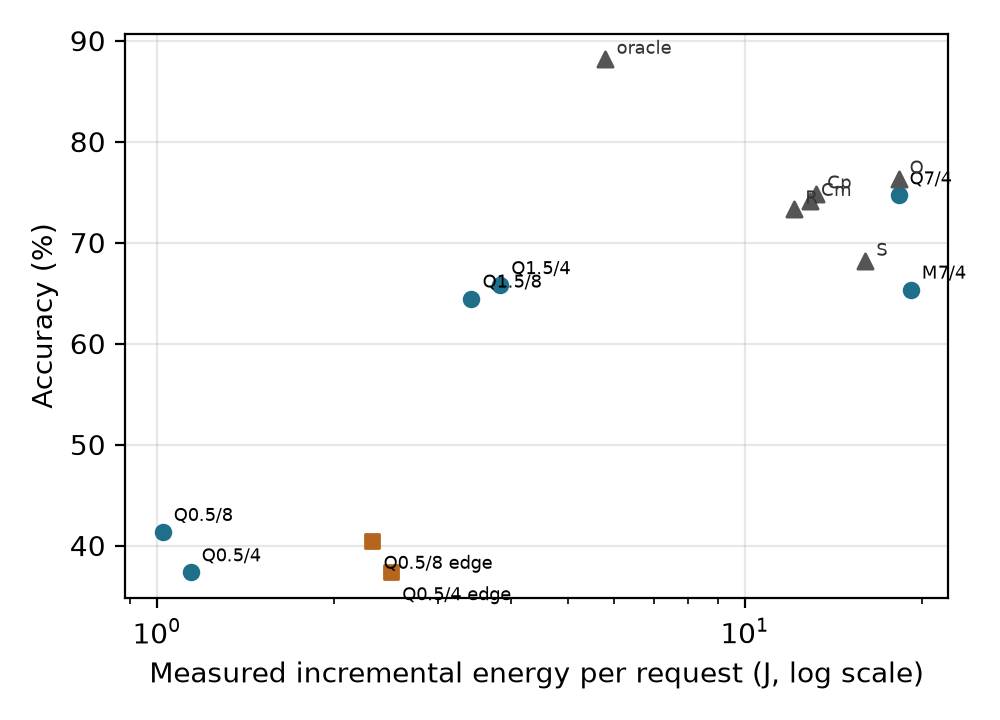
\includegraphics[width=0.85\textwidth]{../results/figures/pareto_energy_accuracy.png}
\caption{Left: accuracy against measured incremental energy per request for every configuration on all 450 items (Q = Qwen2.5, M = Mistral, size/bits; circles GPU, squares emulated CPU edge). Right: the 135 test items, device tier; light circles are single configurations, triangles routing policies with estimated energy (S static rule, Cp and Cm cascades on $p_{\max}$ and margin, R learned router, Opt optimiser, identical to always Q7/4); the hollow triangle is the unattainable oracle.}\label{fig:pareto}
\end{figure*}

\subsection{RQ2: sovereignty scorecard}\label{sec:rq2}
We scored three options on six dimensions with an explicit rubric and cited evidence (\texttt{configs/sovereignty\_inputs.json}). With equal weights the scores were qwen2.5 local (device) 0.79; mistral-7b local (device) 0.75; mistral api, eu endpoint (characterised) 0.42. Across 5000 random weightings drawn uniformly from the simplex, the ranking never changed: qwen2.5 local (device) always ranked 1, mistral-7b local (device) always ranked 2, mistral api, eu endpoint (characterised) always ranked 3. The stability is itself a finding about the instrument, not only about the options: under this rubric the self-hosted options dominate the hosted API on every dimension, so no weighting can reverse them, and the two local options differ only in operational independence (a third-party conversion we could not verify). The rubric deliberately scores the deploying organisation's control, not the model publisher's jurisdiction; an organisation that weighs publisher origin would need an extra dimension, and then the EU-origin model could rank first. Making that choice explicit is the point of the instrument.


\subsection{RQ3: routing}\label{sec:rq3}
\begin{table}[t]\centering\footnotesize
\caption{Routing policies on the 135 held-out test items, device tier. $\Delta$: accuracy change in points versus always Qwen2.5-7B. Saving: mean energy per request saved versus the same baseline.}\label{tab:routing}
\begin{tabular}{@{}lrrr@{}}\toprule
Policy & Acc. & $\Delta$ & Saving\\\midrule
always mistral7b-q4 & 65.2 & -11.1 & -5\%\\
always qwen0.5b-q4 & 38.5 & -37.8 & 94\%\\
always qwen0.5b-q8 & 41.5 & -34.8 & 94\%\\
always qwen1.5b-q4 & 71.9 & -4.4 & 79\%\\
always qwen1.5b-q8 & 69.6 & -6.7 & 81\%\\
always qwen7b-q4 & 76.3 & +0.0 & 0\%\\
static sensitivity rule & 68.1 & -8.1 & 12\%\\
cascade p\_max & 74.8 & -1.5 & 28\%\\
cascade margin & 74.1 & -2.2 & 29\%\\
learned router & 73.3 & -3.0 & 34\%\\
constraint-aware optimiser & 76.3 & +0.0 & 0\%\\
oracle (upper bound, uses labels) & 88.1 & +11.9 & 68\%\\
\bottomrule\end{tabular}\end{table}

Table~\ref{tab:routing} reports all policies on the 135 test items. Always using Qwen2.5-1.5B saved 79\% of energy at -4.4 points. The confidence cascades and the learned router sat in between: the margin cascade saved 29\% at -2.2 points, the $p_{\max}$ cascade 28\% at -1.5, and the learned router 34\% at -3.0. The tuned cascade thresholds were high ($\tau=0.99$ and 0.98), because the small model is confidently wrong on many items, which the pilot had already suggested. The constraint-aware optimiser chose Qwen2.5-7B in every domain: no cheaper single configuration stayed within 5 points of it on validation. The static sensitivity rule, which keeps sensitive items on the EU-origin model, saved 12\% and lost 8.1 points: here sovereignty preferences cost accuracy rather than energy. An oracle that knew which model would be right reached 88.1\% at 68\% saving, showing how much headroom better confidence signals could unlock.

\textbf{H3.} Selected on validation, the cascade margin policy saved 29.3\% of energy per request on test (paired saving 3.7 to 7.0\,J per request, 95\% interval) with an accuracy change of -2.2 points [-5.9, +1.5]. Both point estimates meet the pre-registered thresholds, so H3 is supported on point estimates. However, the lower end of the accuracy interval exceeds the 5-point tolerance, so with 135 test items we cannot rule out a loss larger than we said we would accept. We read this as tentative support.


\textbf{Live validation.} To check the offline replay, the H3 policy was run live on the Mac the next day: both models loaded on the GPU, the 135 test items routed in real time with the validation-tuned $\tau=0.98$, alternating with always-7B blocks over 3 rounds under a fresh 1.13\,W idle baseline. Measured energy per request was 19.7\,J for always-7B and 15.0\,J for the cascade, a measured saving of 23.8\% (per round 23.4, 23.3, 24.8\%), against 29.3\% estimated offline. The cascade escalated 44\% of items live and scored 74.1\% against 76.3\% for always-7B. Measured live, the saving falls below the 25\% threshold in every round, so on measured energy H3 is not supported, and the offline replay overstated the saving. The system recorded 1 memory page-out(s) over the whole live run; we report it but, with both models using a small fraction of 64\,GB, do not treat it as material.


\section{Discussion}
\textbf{What an SME can take from this.} On one laptop, the choice of model moved energy per request by more than an order of magnitude (1.0 to 19.1\,J across configuration means) while moving accuracy by tens of points, and the two did not move together in a simple way: the EU-origin 7B model cost as much as the most accurate model but was no more accurate than a model a fifth of its size. Measured energy, not parameter count, is what separates these options. Placement mattered too: moving the 0.5B models from the laptop GPU to four CPU cores, a stand-in for a modest on-premise server, made them slower and costlier at the same accuracy. ``Running it at the edge'' is therefore not automatically the frugal choice; it depends on the hardware the edge actually has.

\textbf{Why routing helped only modestly.} Routing pays off when a cheap model knows when it is likely to be wrong. Here the small model was often confidently wrong, so to stay near the large model's accuracy the margin cascade had to escalate 44\% of items and still pay for the small model on each of them, and its estimated saving shrank from the 79\% the small model alone offers to 29\%. The gap between the cascades and the oracle shows where the leverage is: better confidence estimation, task-aware routing features or a verifier would convert more of that headroom into savings \cite{guo2017,kadavath2022,hybridllm}. For an SME the practical reading is that routing is worth a meaningful fraction of energy, not most of it, at today's small-model calibration, and that simply using the small model may be the better trade when a few points of accuracy are affordable.

\textbf{Sovereignty as a design decision.} The scorecard's stable ranking came from the rubric, not from the data: once self-hosting is scored as the organisation's own control, every local option beats any hosted one regardless of weights, and the EU-origin model is not favoured. A different organisation could reasonably score publisher jurisdiction, training-data transparency or supply-chain origin more finely and reach a different ranking. We think this is the right way to use such an instrument: as a transparent statement of which dimensions an organisation chooses to value, with evidence attached, rather than as a single objective number. The static sensitivity rule makes the trade-off concrete: honouring a preference for an EU-origin model on sensitive items cost accuracy without saving much energy.

\textbf{What one laptop cannot show.} The continuum in this study is short: one GPU, its own CPU and a documented but unexecuted cloud tier. The figures say nothing about data-centre efficiency, batching servers or network energy, and the edge tier shares the chip with the device tier. The contribution is a method and a calibrated first data point that a larger study can extend to real edge hardware and hosted tiers.


\section{Threats to validity}
\textbf{Construct.} Multiple-choice accuracy with first-token scoring measures recognition, not the open-ended generation many SME tasks need. MMLU subjects are proxies for sector tasks. Component power from \texttt{powermetrics} omits display, memory and supply losses, and even apportioning within a cell hides per-item variation. The sovereignty scores apply the author's rubric to cited evidence; the rubric itself is a normative choice, which is why we test weight sensitivity.

\textbf{Internal.} The edge tier shares the chip, memory and thermal envelope with the device tier, so it is an emulation, not separate hardware. Thermal state and background activity can drift during a run; we log both and replay a timing subset, but cannot exclude all drift. The Mistral file is a third-party conversion whose source revision we did not verify.

\textbf{External.} One machine, one runtime, small models and three domains. Results may not transfer to other accelerators, larger models, batching servers or real enterprise traffic.

\textbf{Conclusion.} 135 test items per policy comparison give intervals of several points on accuracy. H3 is the single confirmatory test; all other comparisons are descriptive.

\section{Future work}\label{sec:future}
A PhD-scale version of this study would (i) meter real edge hardware and a hosted tier with wall-plug instruments, so device, edge and cloud energy share one method; (ii) move from multiple-choice probes to open-ended tasks with calibrated evaluation in the digital-industry, automotive and healthcare settings named in the f-inference project; (iii) treat placement as an online decision across many devices and providers, where routing must also respect data-sharing agreements between organisations; and (iv) test the sovereignty instrument with SMEs and policy experts, asking which dimensions they actually trade against energy and quality.

\clearpage
\appendix
\section{Additional tables}
\begin{table}[h]\centering\footnotesize
\caption{Accuracy (\%) by domain and configuration, 150 items per domain.}\label{tab:domain}
\begin{tabular}{@{}llrrr@{}}\toprule
Config & Tier & Health & Digital ind. & Control\\\midrule
mistral7b-q4 & device & 61.3 & 60.0 & 74.7\\
qwen0.5b-q4 & device & 24.0 & 43.3 & 44.7\\
qwen0.5b-q4 & edge & 24.0 & 43.3 & 44.7\\
qwen0.5b-q8 & device & 26.7 & 50.0 & 47.3\\
qwen0.5b-q8 & edge & 27.3 & 48.0 & 46.0\\
qwen1.5b-q4 & device & 62.7 & 58.7 & 76.0\\
qwen1.5b-q4 & edge & 62.7 & 58.7 & 76.0\\
qwen1.5b-q8 & device & 62.0 & 56.0 & 75.3\\
qwen7b-q4 & device & 58.7 & 74.0 & 91.3\\
\bottomrule\end{tabular}\end{table}
\begin{table}[h]\centering\footnotesize
\caption{Energy per request (J) by cell, with the idle-window alternatives (first and last 30\,s of the baseline). Swapped cells are excluded.}\label{tab:cells}
\begin{tabular}{@{}lrrrr@{}}\toprule
Cell & Power (W) & J/req & idle first & idle last\\\midrule
mistral7b-q4 d digi & 47.8 & 12.26 & 12.32 & 12.20\\
mistral7b-q4 d gene & 48.5 & 11.97 & 12.02 & 11.91\\
mistral7b-q4 d heal & 51.1 & 33.20 & 33.36 & 33.05\\
qwen0.5b-q4 d digi & 29.3 & 0.84 & 0.84 & 0.83\\
qwen0.5b-q4 d gene & 28.4 & 0.79 & 0.80 & 0.78\\
qwen0.5b-q4 d heal & 36.1 & 1.80 & 1.81 & 1.78\\
qwen0.5b-q4 e digi & 12.9 & 1.82 & 1.86 & 1.78\\
qwen0.5b-q4 e gene & 13.4 & 1.89 & 1.92 & 1.85\\
qwen0.5b-q4 e heal & 15.4 & 3.80 & 3.86 & 3.74\\
qwen0.5b-q8 d digi & 28.7 & 0.73 & 0.74 & 0.73\\
qwen0.5b-q8 d gene & 27.1 & 0.67 & 0.68 & 0.66\\
qwen0.5b-q8 d heal & 37.7 & 1.66 & 1.68 & 1.65\\
qwen0.5b-q8 e digi & 11.8 & 1.58 & 1.61 & 1.55\\
qwen0.5b-q8 e gene & 12.3 & 1.67 & 1.70 & 1.63\\
qwen0.5b-q8 e heal & 15.2 & 3.73 & 3.79 & 3.67\\
qwen1.5b-q4 d digi & 38.9 & 2.72 & 2.74 & 2.70\\
qwen1.5b-q4 d gene & 38.6 & 2.59 & 2.60 & 2.57\\
qwen1.5b-q4 d heal & 44.9 & 6.19 & 6.23 & 6.16\\
qwen1.5b-q4 e digi & \multicolumn{4}{c}{excluded (page-outs)}\\
qwen1.5b-q4 e gene & 14.1 & 6.09 & 6.20 & 5.98\\
qwen1.5b-q4 e heal & \multicolumn{4}{c}{excluded (page-outs)}\\
qwen1.5b-q8 d digi & 38.5 & 2.37 & 2.38 & 2.35\\
qwen1.5b-q8 d gene & 38.7 & 2.28 & 2.30 & 2.27\\
qwen1.5b-q8 d heal & 46.4 & 5.63 & 5.66 & 5.60\\
qwen7b-q4 d digi & 47.2 & 12.71 & 12.77 & 12.64\\
qwen7b-q4 d gene & 47.2 & 12.24 & 12.30 & 12.18\\
qwen7b-q4 d heal & 50.6 & 29.81 & 29.95 & 29.67\\
\bottomrule\end{tabular}\end{table}


\section*{Reproducibility}
Items, protocol, model pins, raw per-request rows, cell manifests, the \texttt{powermetrics} log and analysis code are committed. \texttt{python scripts/analyze\_mac.py} regenerates every table, the figure and every generated paragraph in this report (results, routing, sovereignty, discussion and the abstract's results sentence) from those records; the method and related-work text is written by hand. The Mac run script and its log are included.

\section*{AI-assistance statement}
This project was built with AI coding assistants under the author's direction. The author set the research direction and scope and ran the benchmark on his own laptop. AI assistants proposed the protocol, wrote most of the code, documentation and this report's first draft, and ran the analysis. The author's final review of the wording is the last step before release. The work is independent and not affiliated with or endorsed by TU Delft or the f-inference consortium.

\small
\begin{thebibliography}{99}
\bibitem{ding2022roadmap} A.~Y. Ding, E.~Peltonen, T.~Meuser et al. Roadmap for edge AI: A Dagstuhl perspective. arXiv:2112.00616, 2021.
\bibitem{katare2023} D.~Katare, D.~Perino, J.~Nurmi, M.~Warnier, M.~Janssen, A.~Y. Ding. A survey on approximate edge AI for energy efficient autonomous driving services. arXiv:2304.14271, 2023.
\bibitem{varghese2021} B.~Varghese, E.~de Lara, A.~Y. Ding et al. Revisiting the arguments for edge computing research. doi:10.1109/MIC.2021.3093924
\bibitem{satya2017} M.~Satyanarayanan. The emergence of edge computing. doi:10.1109/MC.2017.9
\bibitem{shi2016} W.~Shi, J.~Cao, Q.~Zhang, Y.~Li, L.~Xu. Edge computing: Vision and challenges. doi:10.1109/JIOT.2016.2579198
\bibitem{deng2020} S.~Deng et al. Edge intelligence: The confluence of edge computing and artificial intelligence. doi:10.1109/JIOT.2020.2984887
\bibitem{frugalgpt} L.~Chen, M.~Zaharia, J.~Zou. FrugalGPT: How to use large language models while reducing cost and improving performance. arXiv:2305.05176, 2023.
\bibitem{routellm} I.~Ong et al. RouteLLM: Learning to route LLMs with preference data. arXiv:2406.18665, 2024.
\bibitem{hybridllm} D.~Ding et al. Hybrid LLM: Cost-efficient and quality-aware query routing. arXiv:2404.14618, 2024.
\bibitem{strubell2019} E.~Strubell, A.~Ganesh, A.~McCallum. Energy and policy considerations for deep learning in NLP. doi:10.18653/v1/P19-1355
\bibitem{schwartz2020} R.~Schwartz, J.~Dodge, N.~A. Smith, O.~Etzioni. Green AI. doi:10.1145/3381831
\bibitem{patterson2021} D.~Patterson et al. Carbon emissions and large neural network training. arXiv:2104.10350, 2021.
\bibitem{luccioni2024} S.~Luccioni, Y.~Jernite, E.~Strubell. Power hungry processing: Watts driving the cost of AI deployment? doi:10.1145/3630106.3658542
\bibitem{samsi2023} S.~Samsi et al. From words to watts: Benchmarking the energy costs of large language model inference. arXiv:2310.03003, 2023.
\bibitem{lannelongue2021} L.~Lannelongue, J.~Grealey, M.~Inouye. Green algorithms: Quantifying the carbon footprint of computation. doi:10.1002/advs.202100707
\bibitem{henderson2020} P.~Henderson et al. Towards the systematic reporting of the energy and carbon footprints of machine learning. arXiv:2002.05651, 2020.
\bibitem{wu2022} C.-J. Wu et al. Sustainable AI: Environmental implications, challenges and opportunities. arXiv:2111.00364, 2021.
\bibitem{dettmers2022} T.~Dettmers, M.~Lewis, Y.~Belkada, L.~Zettlemoyer. LLM.int8(): 8-bit matrix multiplication for transformers at scale. arXiv:2208.07339, 2022.
\bibitem{frantar2022} E.~Frantar, S.~Ashkboos, T.~Hoefler, D.~Alistarh. GPTQ: Accurate post-training quantization for generative pre-trained transformers. arXiv:2210.17323, 2022.
\bibitem{lin2023} J.~Lin et al. AWQ: Activation-aware weight quantization for LLM compression and acceleration. arXiv:2306.00978, 2023.
\bibitem{pope2022} R.~Pope et al. Efficiently scaling transformer inference. arXiv:2211.05102, 2022.
\bibitem{kadavath2022} S.~Kadavath et al. Language models (mostly) know what they know. arXiv:2207.05221, 2022.
\bibitem{guo2017} C.~Guo, G.~Pleiss, Y.~Sun, K.~Q. Weinberger. On calibration of modern neural networks. arXiv:1706.04599, 2017.
\bibitem{mmlu} D.~Hendrycks et al. Measuring massive multitask language understanding. arXiv:2009.03300, 2020.
\bibitem{pubmedqa} Q.~Jin, B.~Dhingra, Z.~Liu, W.~Cohen, X.~Lu. PubMedQA: A dataset for biomedical research question answering. arXiv:1909.06146, 2019.
\bibitem{arc} P.~Clark et al. Think you have solved question answering? Try ARC, the AI2 reasoning challenge. arXiv:1803.05457, 2018.
\bibitem{qwen25} Qwen Team. Qwen2.5 technical report. arXiv:2412.15115, 2024.
\bibitem{mistral7b} A.~Q. Jiang et al. Mistral 7B. arXiv:2310.06825, 2023.
\bibitem{esposito2026} M.~Esposito, L.~Marchesi, R.~Tonelli, V.~Lenarduzzi. Sovereign-by-design: A reference architecture for AI and blockchain enabled systems. arXiv:2602.05486, 2026.
\bibitem{canqa} CAN-QA: A question-answering benchmark for reasoning over in-vehicle CAN traffic. arXiv:2604.24935, 2026.
\bibitem{dingtrust2021} A.~Y. Ding, M.~Janssen, J.~Crowcroft. Trustworthy and sustainable edge AI: A research agenda. doi:10.1109/TPSISA52974.2021.00019
\end{thebibliography}

\end{document}
